\documentclass{standalone}
\usepackage{tikz}
\usetikzlibrary{patterns, positioning}
\usepackage[sfdefault]{ClearSans} %% option 'sfdefault' activates Clear Sans as the default text font
\usepackage[T1]{fontenc}

\begin{document}
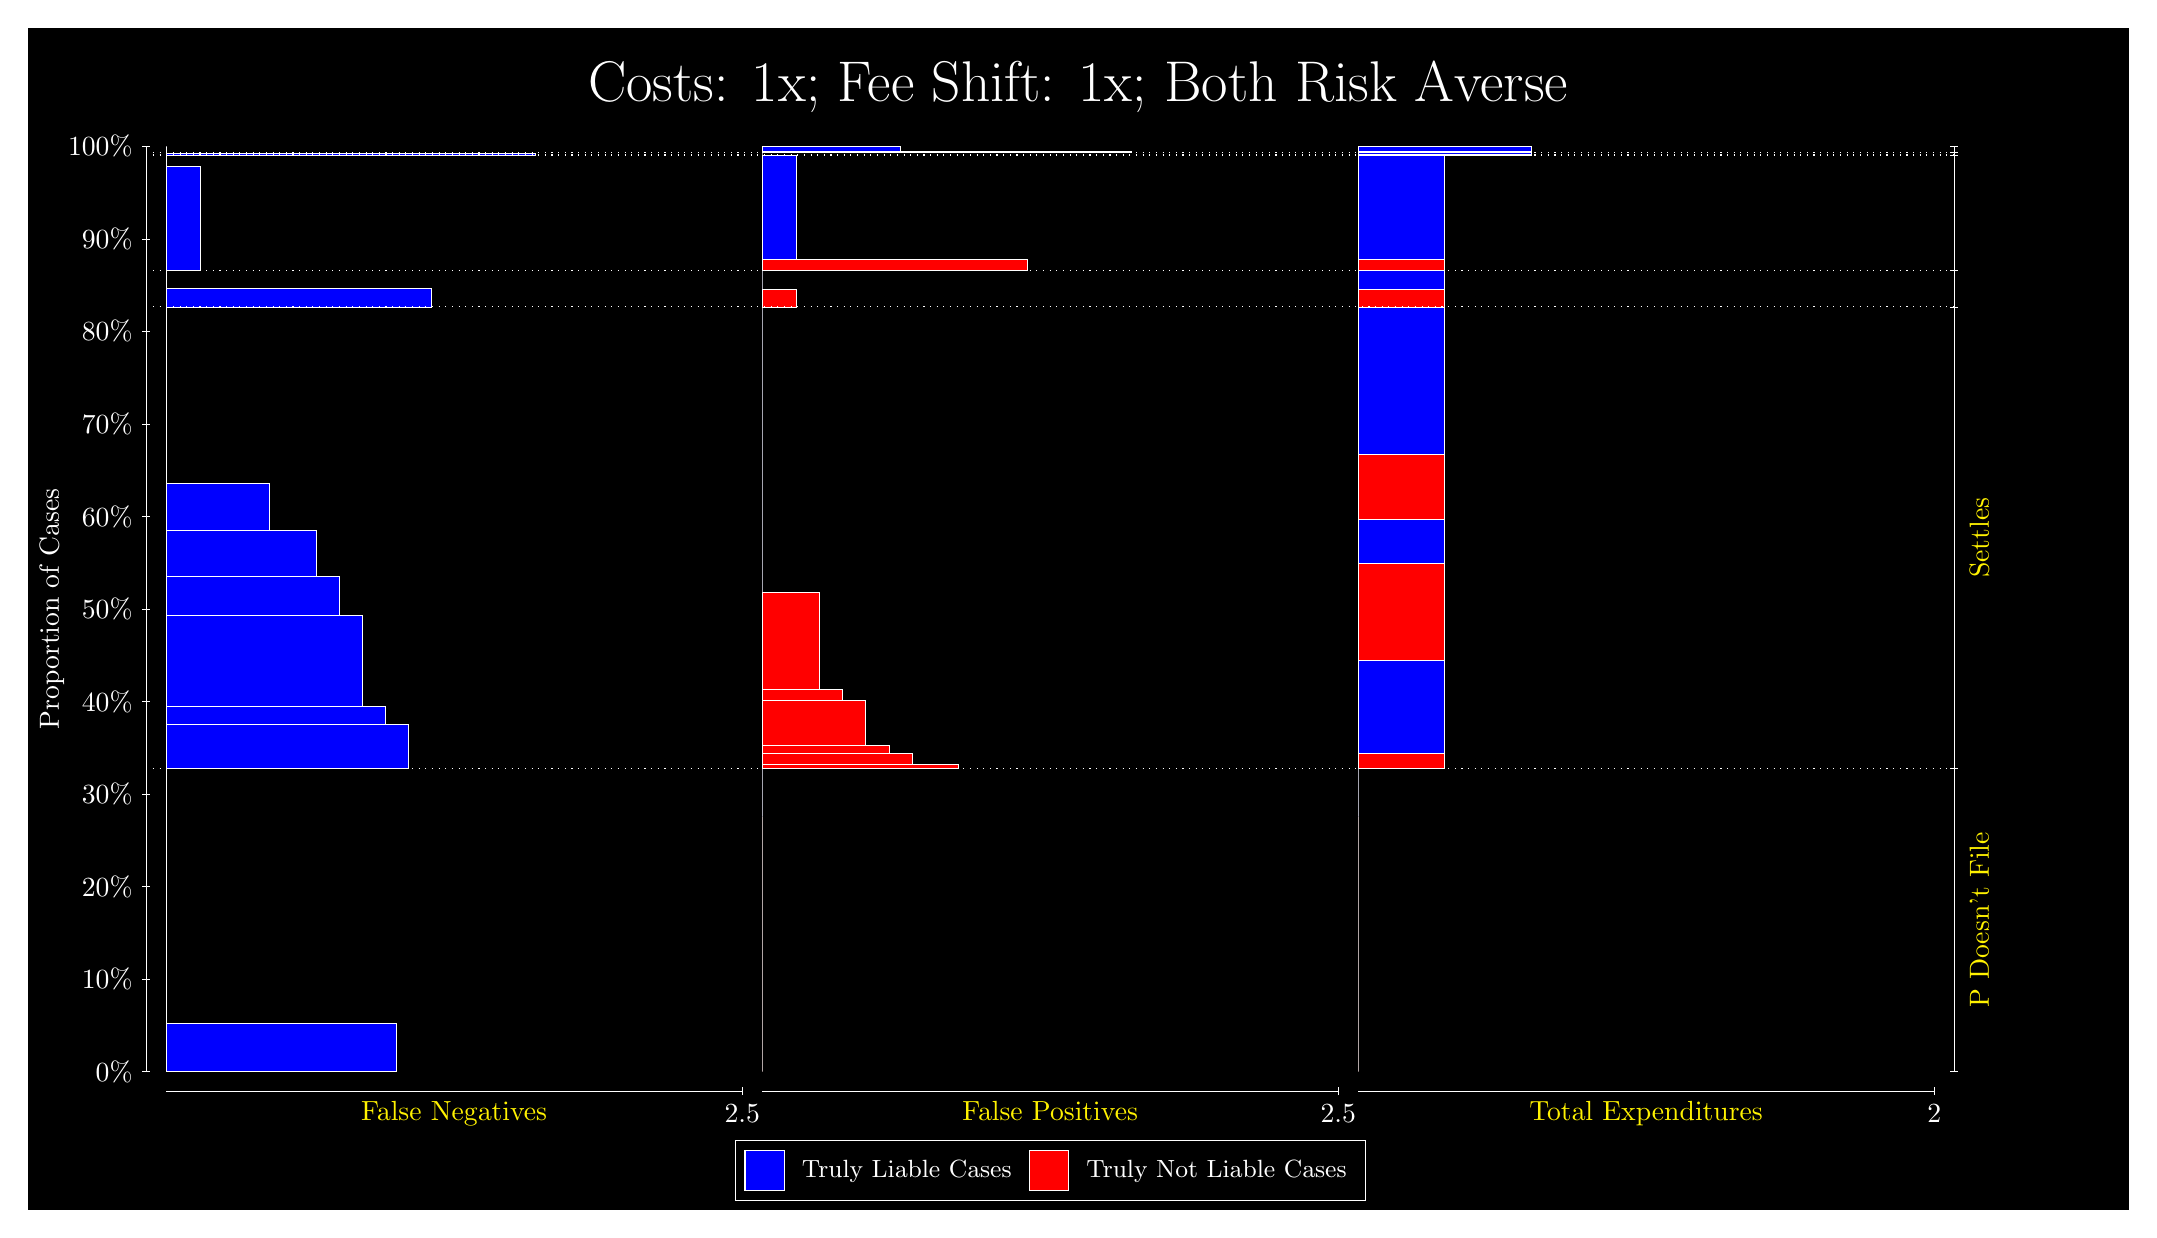
\begin{tikzpicture}
\draw[fill=black] (0,0) rectangle (26.667,15);
\draw[text=white] (0,13.5) rectangle (26.667,15) node[midway] {\huge Costs: 1x; Fee Shift: 1x; Both Risk Averse};
\draw[white, very thin] (1.5,1.75) -- (1.5,13.5);
\node[rotate=90, text=white, anchor=center] at (0.3, 7.625) {Proportion of Cases};
\draw[white, very thin] (1.45,1.75) -- (1.55,1.75);
\node[text=white, anchor=east] at (1.45, 1.75) {0\%};
\draw[white, very thin] (1.45,2.925) -- (1.55,2.925);
\node[text=white, anchor=east] at (1.45, 2.925) {10\%};
\draw[white, very thin] (1.45,4.1) -- (1.55,4.1);
\node[text=white, anchor=east] at (1.45, 4.1) {20\%};
\draw[white, very thin] (1.45,5.275) -- (1.55,5.275);
\node[text=white, anchor=east] at (1.45, 5.275) {30\%};
\draw[white, very thin] (1.45,6.45) -- (1.55,6.45);
\node[text=white, anchor=east] at (1.45, 6.45) {40\%};
\draw[white, very thin] (1.45,7.625) -- (1.55,7.625);
\node[text=white, anchor=east] at (1.45, 7.625) {50\%};
\draw[white, very thin] (1.45,8.8) -- (1.55,8.8);
\node[text=white, anchor=east] at (1.45, 8.8) {60\%};
\draw[white, very thin] (1.45,9.975) -- (1.55,9.975);
\node[text=white, anchor=east] at (1.45, 9.975) {70\%};
\draw[white, very thin] (1.45,11.15) -- (1.55,11.15);
\node[text=white, anchor=east] at (1.45, 11.15) {80\%};
\draw[white, very thin] (1.45,12.325) -- (1.55,12.325);
\node[text=white, anchor=east] at (1.45, 12.325) {90\%};
\draw[white, very thin] (1.45,13.5) -- (1.55,13.5);
\node[text=white, anchor=east] at (1.45, 13.5) {100\%};

\draw[white, very thin] (24.457,1.75) -- (24.457,13.5);
\draw[white, very thin] (24.407,1.75) -- (24.507,1.75);
\node[anchor=west] at (24.407, 1.75) {};
\draw[white, very thin] (24.407,5.6) -- (24.507,5.6);
\node[anchor=west] at (24.407, 5.6) {};
\draw[white, very thin] (24.407,11.461) -- (24.507,11.461);
\node[anchor=west] at (24.407, 11.461) {};
\draw[white, very thin] (24.407,11.924) -- (24.507,11.924);
\node[anchor=west] at (24.407, 11.924) {};
\draw[white, very thin] (24.407,13.39) -- (24.507,13.39);
\node[anchor=west] at (24.407, 13.39) {};
\draw[white, very thin] (24.407,13.422) -- (24.507,13.422);
\node[anchor=west] at (24.407, 13.422) {};
\draw[white, very thin] (24.407,13.5) -- (24.507,13.5);
\node[anchor=west] at (24.407, 13.5) {};

\draw[white, very thin, fill=blue] (1.75,1.75) rectangle (4.6775,2.3639);
\draw[white, very thin, fill=red] (1.75,2.3639) rectangle (1.75,5.6);
\draw[white, very thin, fill=blue] (1.75,5.6) rectangle (4.8239,6.1656);
\draw[white, very thin, fill=blue] (1.75,6.1656) rectangle (4.5312,6.3829);
\draw[white, very thin, fill=blue] (1.75,6.3829) rectangle (4.2384,7.5415);
\draw[white, very thin, fill=blue] (1.75,7.5415) rectangle (3.9457,8.0402);
\draw[white, very thin, fill=blue] (1.75,8.0402) rectangle (3.6529,8.6289);
\draw[white, very thin, fill=blue] (1.75,8.6289) rectangle (3.0674,9.2227);
\draw[white, very thin, fill=red] (1.75,9.2227) rectangle (1.75,11.461);
\draw[white, very thin, fill=blue] (1.75,11.461) rectangle (5.1167,11.697);
\draw[white, very thin, fill=red] (1.75,11.697) rectangle (1.75,11.924);
\draw[white, very thin, fill=blue] (1.75,11.924) rectangle (2.1891,13.248);
\draw[white, very thin, fill=red] (1.75,13.248) rectangle (1.75,13.39);
\draw[white, very thin, fill=blue] (1.75,13.39) rectangle (6.4341,13.407);
\draw[white, very thin, fill=red] (1.75,13.407) rectangle (1.75,13.422);
\draw[white, very thin, fill=red] (1.75,13.422) rectangle (1.75,13.438);
\draw[white, very thin, fill=blue] (1.75,13.438) rectangle (1.75,13.5);
\draw[white, very thin, fill=red] (9.3189,1.75) rectangle (9.3189,4.9861);
\draw[white, very thin, fill=blue] (9.3189,4.9861) rectangle (9.3189,5.6);
\draw[white, very thin, fill=red] (9.3189,5.6) rectangle (11.807,5.6567);
\draw[white, very thin, fill=red] (9.3189,5.6567) rectangle (11.222,5.7867);
\draw[white, very thin, fill=red] (9.3189,5.7867) rectangle (10.929,5.8974);
\draw[white, very thin, fill=red] (9.3189,5.8974) rectangle (10.636,6.4711);
\draw[white, very thin, fill=red] (9.3189,6.4711) rectangle (10.344,6.6087);
\draw[white, very thin, fill=red] (9.3189,6.6087) rectangle (10.051,7.8382);
\draw[white, very thin, fill=blue] (9.3189,7.8382) rectangle (9.3189,11.461);
\draw[white, very thin, fill=red] (9.3189,11.461) rectangle (9.758,11.688);
\draw[white, very thin, fill=blue] (9.3189,11.688) rectangle (9.3189,11.924);
\draw[white, very thin, fill=red] (9.3189,11.924) rectangle (12.686,12.066);
\draw[white, very thin, fill=blue] (9.3189,12.066) rectangle (9.758,13.39);
\draw[white, very thin, fill=red] (9.3189,13.39) rectangle (9.3189,13.405);
\draw[white, very thin, fill=blue] (9.3189,13.405) rectangle (9.3189,13.422);
\draw[white, very thin, fill=red] (9.3189,13.422) rectangle (14.003,13.438);
\draw[white, very thin, fill=blue] (9.3189,13.438) rectangle (11.075,13.5);
\draw[white, very thin, fill=red] (16.888,1.75) rectangle (16.888,4.9861);
\draw[white, very thin, fill=blue] (16.888,4.9861) rectangle (16.888,5.6);
\draw[white, very thin, fill=red] (16.888,5.6) rectangle (17.986,5.7867);
\draw[white, very thin, fill=blue] (16.888,5.7867) rectangle (17.986,6.9692);
\draw[white, very thin, fill=red] (16.888,6.9692) rectangle (17.986,8.1987);
\draw[white, very thin, fill=blue] (16.888,8.1987) rectangle (17.986,8.7643);
\draw[white, very thin, fill=red] (16.888,8.7643) rectangle (17.986,9.5863);
\draw[white, very thin, fill=blue] (16.888,9.5863) rectangle (17.986,11.461);
\draw[white, very thin, fill=red] (16.888,11.461) rectangle (17.986,11.688);
\draw[white, very thin, fill=blue] (16.888,11.688) rectangle (17.986,11.924);
\draw[white, very thin, fill=red] (16.888,11.924) rectangle (17.986,12.066);
\draw[white, very thin, fill=blue] (16.888,12.066) rectangle (17.986,13.39);
\draw[white, very thin, fill=red] (16.888,13.39) rectangle (19.083,13.405);
\draw[white, very thin, fill=blue] (16.888,13.405) rectangle (19.083,13.422);
\draw[white, very thin, fill=red] (16.888,13.422) rectangle (19.083,13.438);
\draw[white, very thin, fill=blue] (16.888,13.438) rectangle (19.083,13.5);
\draw[white, dotted] (1.5,5.6) -- (24.457,5.6);
\draw[white, dotted] (1.5,11.461) -- (24.457,11.461);
\draw[white, dotted] (1.5,11.924) -- (24.457,11.924);
\draw[white, dotted] (1.5,13.39) -- (24.457,13.39);
\draw[white, dotted] (1.5,13.422) -- (24.457,13.422);
\draw[white, very thin] (1.75,1.5) -- (9.0689,1.5);
\node[text=yellow, anchor=north] at (5.4094, 1.5) {False Negatives};
\draw[white, very thin] (9.0689,1.45) -- (9.0689,1.55);
\node[text=white, anchor=north] at (9.0689, 1.45) {2.5};

\draw[white, very thin] (9.3189,1.5) -- (16.638,1.5);
\node[text=yellow, anchor=north] at (12.978, 1.5) {False Positives};
\draw[white, very thin] (16.638,1.45) -- (16.638,1.55);
\node[text=white, anchor=north] at (16.638, 1.45) {2.5};

\draw[white, very thin] (16.888,1.5) -- (24.207,1.5);
\node[text=yellow, anchor=north] at (20.547, 1.5) {Total Expenditures};
\draw[white, very thin] (24.207,1.45) -- (24.207,1.55);
\node[text=white, anchor=north] at (24.207, 1.45) {2};

\node[text=yellow, centered, rotate=90] at (24.777, 3.675) {P Doesn't File};
\node[text=yellow, centered, rotate=90] at (24.777, 8.5304) {Settles};





\draw (12.978300999999998,1.5) node[draw=none] (baseCoordinate) {};
\begin{scope}[align=center]
        \matrix[scale=0.5, draw=white, below=0.5cm of baseCoordinate, nodes={draw}, column sep=0.1cm]{
            \node[rectangle, draw, minimum width=0.5cm, minimum height=0.5cm, fill=blue] {}; &
            \node[draw=none, font=\small, text=white] (B) {Truly Liable Cases}; &
            \node[rectangle, draw, minimum width=0.5cm, minimum height=0.5cm, fill=red] {}; &
            \node[draw=none, font=\small, text=white] (B) {Truly Not Liable Cases}; \\
            };
\end{scope}

\end{tikzpicture}
\end{document}